\documentclass[journal]{IEEEtran}
% IEEE Open Journal of Vehicular Technology submission.  At submission, move
% the body into the official OJVT template (ieeeoj.cls); the content and
% bibliography are template-independent.
\usepackage{amsmath,amssymb,amsthm}
\usepackage{graphicx}
\usepackage{booktabs,multirow,array,tabularx}
\usepackage{algorithm}
\usepackage{algpseudocode}
\usepackage{tikz}
\usepackage{pgfplots}
\usepackage{pgfplotstable}
\usepgfplotslibrary{groupplots}
\usetikzlibrary{arrows.meta,positioning,fit,calc,shapes.geometric}
\pgfplotsset{compat=1.18}
\usepackage{xcolor}
\usepackage{url}
\usepackage{cite}
\usepackage{balance}
\usepackage{microtype}

% ---- Results: every number comes from results/v2 (scripts/analyze_campaign_v2.py)
\newcommand{\resdir}{../results/v2}
\newcommand{\TBD}{\textcolor{red}{[run]}}
\IfFileExists{\resdir/macros.tex}{\input{\resdir/macros.tex}}{}
% Fallbacks for result macros; real values come from results/v2/macros.tex
\providecommand{\resBoxModeOnlyAoi}{\TBD}
\providecommand{\resBoxModeOnlyApBevFiveZero}{\TBD}
\providecommand{\resBoxModeOnlyApThreeDSevenZero}{\TBD}
\providecommand{\resBoxModeOnlyBackgroundDelivery}{\TBD}
\providecommand{\resBoxModeOnlyCertCondMiss}{\TBD}
\providecommand{\resBoxModeOnlyCertObjectMiss}{\TBD}
\providecommand{\resBoxModeOnlyCertWindowMiss}{\TBD}
\providecommand{\resBoxModeOnlyCriticalAwareness}{\TBD}
\providecommand{\resBoxModeOnlyDecisionMs}{\TBD}
\providecommand{\resBoxModeOnlyHiddenAwareness}{\TBD}
\providecommand{\resBoxModeOnlyKbps}{\TBD}
\providecommand{\resCertischedAoi}{\TBD}
\providecommand{\resCertischedApBevFiveZero}{\TBD}
\providecommand{\resCertischedApThreeDSevenZero}{\TBD}
\providecommand{\resCertischedBackgroundDelivery}{\TBD}
\providecommand{\resCertischedCertCondMiss}{\TBD}
\providecommand{\resCertischedCertObjectMiss}{\TBD}
\providecommand{\resCertischedCertWindowMiss}{\TBD}
\providecommand{\resCertischedCriticalAwareness}{\TBD}
\providecommand{\resCertischedDecisionMs}{\TBD}
\providecommand{\resCertischedGreedyAoi}{\TBD}
\providecommand{\resCertischedGreedyApBevFiveZero}{\TBD}
\providecommand{\resCertischedGreedyApThreeDSevenZero}{\TBD}
\providecommand{\resCertischedGreedyBackgroundDelivery}{\TBD}
\providecommand{\resCertischedGreedyCertCondMiss}{\TBD}
\providecommand{\resCertischedGreedyCertObjectMiss}{\TBD}
\providecommand{\resCertischedGreedyCertWindowMiss}{\TBD}
\providecommand{\resCertischedGreedyCriticalAwareness}{\TBD}
\providecommand{\resCertischedGreedyDecisionMs}{\TBD}
\providecommand{\resCertischedGreedyHiddenAwareness}{\TBD}
\providecommand{\resCertischedGreedyKbps}{\TBD}
\providecommand{\resCertischedHiddenAwareness}{\TBD}
\providecommand{\resCertischedKbps}{\TBD}
\providecommand{\resConfidenceDensityAoi}{\TBD}
\providecommand{\resConfidenceDensityApBevFiveZero}{\TBD}
\providecommand{\resConfidenceDensityApThreeDSevenZero}{\TBD}
\providecommand{\resConfidenceDensityBackgroundDelivery}{\TBD}
\providecommand{\resConfidenceDensityCertCondMiss}{\TBD}
\providecommand{\resConfidenceDensityCertObjectMiss}{\TBD}
\providecommand{\resConfidenceDensityCertWindowMiss}{\TBD}
\providecommand{\resConfidenceDensityCriticalAwareness}{\TBD}
\providecommand{\resConfidenceDensityDecisionMs}{\TBD}
\providecommand{\resConfidenceDensityHiddenAwareness}{\TBD}
\providecommand{\resConfidenceDensityKbps}{\TBD}
\providecommand{\resDataGtCritical}{\TBD}
\providecommand{\resDataGtHidden}{\TBD}
\providecommand{\resDataInfrastructureFrames}{\TBD}
\providecommand{\resDataLinks}{\TBD}
\providecommand{\resDataScenarios}{\TBD}
\providecommand{\resDataSequences}{\TBD}
\providecommand{\resDataVehicleFrames}{\TBD}
\providecommand{\resDataWindows}{\TBD}
\providecommand{\resEnvAciAOneZeroEff}{\TBD}
\providecommand{\resEnvAciAOneZeroMiss}{\TBD}
\providecommand{\resEnvAciATwoZeroEff}{\TBD}
\providecommand{\resEnvAciATwoZeroMiss}{\TBD}
\providecommand{\resEnvAciAZeroFiveEff}{\TBD}
\providecommand{\resEnvAciAZeroFiveMiss}{\TBD}
\providecommand{\resEnvAciAZeroOneEff}{\TBD}
\providecommand{\resEnvAciAZeroOneMiss}{\TBD}
\providecommand{\resEnvAciAZeroTwoEff}{\TBD}
\providecommand{\resEnvAciAZeroTwoMiss}{\TBD}
\providecommand{\resEnvLastMiss}{\TBD}
\providecommand{\resEnvPointMiss}{\TBD}
\providecommand{\resEnvRollingAOneZeroEff}{\TBD}
\providecommand{\resEnvRollingAOneZeroMiss}{\TBD}
\providecommand{\resEnvRollingATwoZeroEff}{\TBD}
\providecommand{\resEnvRollingATwoZeroMiss}{\TBD}
\providecommand{\resEnvRollingAZeroFiveEff}{\TBD}
\providecommand{\resEnvRollingAZeroFiveMiss}{\TBD}
\providecommand{\resEnvRollingAZeroOneEff}{\TBD}
\providecommand{\resEnvRollingAZeroOneMiss}{\TBD}
\providecommand{\resEnvRollingAZeroTwoEff}{\TBD}
\providecommand{\resEnvRollingAZeroTwoMiss}{\TBD}
\providecommand{\resEnvSplitAOneZeroEff}{\TBD}
\providecommand{\resEnvSplitAOneZeroMiss}{\TBD}
\providecommand{\resEnvSplitATwoZeroEff}{\TBD}
\providecommand{\resEnvSplitATwoZeroMiss}{\TBD}
\providecommand{\resEnvSplitAZeroFiveEff}{\TBD}
\providecommand{\resEnvSplitAZeroFiveMiss}{\TBD}
\providecommand{\resEnvSplitAZeroOneEff}{\TBD}
\providecommand{\resEnvSplitAZeroOneMiss}{\TBD}
\providecommand{\resEnvSplitAZeroTwoEff}{\TBD}
\providecommand{\resEnvSplitAZeroTwoMiss}{\TBD}
\providecommand{\resEtsiCpmRulesAoi}{\TBD}
\providecommand{\resEtsiCpmRulesApBevFiveZero}{\TBD}
\providecommand{\resEtsiCpmRulesApThreeDSevenZero}{\TBD}
\providecommand{\resEtsiCpmRulesBackgroundDelivery}{\TBD}
\providecommand{\resEtsiCpmRulesCertCondMiss}{\TBD}
\providecommand{\resEtsiCpmRulesCertObjectMiss}{\TBD}
\providecommand{\resEtsiCpmRulesCertWindowMiss}{\TBD}
\providecommand{\resEtsiCpmRulesCriticalAwareness}{\TBD}
\providecommand{\resEtsiCpmRulesDecisionMs}{\TBD}
\providecommand{\resEtsiCpmRulesHiddenAwareness}{\TBD}
\providecommand{\resEtsiCpmRulesKbps}{\TBD}
\providecommand{\resFixedLevelRollingAoi}{\TBD}
\providecommand{\resFixedLevelRollingApBevFiveZero}{\TBD}
\providecommand{\resFixedLevelRollingApThreeDSevenZero}{\TBD}
\providecommand{\resFixedLevelRollingBackgroundDelivery}{\TBD}
\providecommand{\resFixedLevelRollingCertCondMiss}{\TBD}
\providecommand{\resFixedLevelRollingCertObjectMiss}{\TBD}
\providecommand{\resFixedLevelRollingCertWindowMiss}{\TBD}
\providecommand{\resFixedLevelRollingCriticalAwareness}{\TBD}
\providecommand{\resFixedLevelRollingDecisionMs}{\TBD}
\providecommand{\resFixedLevelRollingHiddenAwareness}{\TBD}
\providecommand{\resFixedLevelRollingKbps}{\TBD}
\providecommand{\resLastValueBudgetAoi}{\TBD}
\providecommand{\resLastValueBudgetApBevFiveZero}{\TBD}
\providecommand{\resLastValueBudgetApThreeDSevenZero}{\TBD}
\providecommand{\resLastValueBudgetBackgroundDelivery}{\TBD}
\providecommand{\resLastValueBudgetCertCondMiss}{\TBD}
\providecommand{\resLastValueBudgetCertObjectMiss}{\TBD}
\providecommand{\resLastValueBudgetCertWindowMiss}{\TBD}
\providecommand{\resLastValueBudgetCriticalAwareness}{\TBD}
\providecommand{\resLastValueBudgetDecisionMs}{\TBD}
\providecommand{\resLastValueBudgetHiddenAwareness}{\TBD}
\providecommand{\resLastValueBudgetKbps}{\TBD}
\providecommand{\resLinks}{\TBD}
\providecommand{\resMaxWeightAoiAheadOfBgAoi}{\TBD}
\providecommand{\resMaxWeightAoiAheadOfBgApBevFiveZero}{\TBD}
\providecommand{\resMaxWeightAoiAheadOfBgApThreeDSevenZero}{\TBD}
\providecommand{\resMaxWeightAoiAheadOfBgBackgroundDelivery}{\TBD}
\providecommand{\resMaxWeightAoiAheadOfBgCertCondMiss}{\TBD}
\providecommand{\resMaxWeightAoiAheadOfBgCertObjectMiss}{\TBD}
\providecommand{\resMaxWeightAoiAheadOfBgCertWindowMiss}{\TBD}
\providecommand{\resMaxWeightAoiAheadOfBgCriticalAwareness}{\TBD}
\providecommand{\resMaxWeightAoiAheadOfBgDecisionMs}{\TBD}
\providecommand{\resMaxWeightAoiAheadOfBgHiddenAwareness}{\TBD}
\providecommand{\resMaxWeightAoiAheadOfBgKbps}{\TBD}
\providecommand{\resMaxWeightAoiAoi}{\TBD}
\providecommand{\resMaxWeightAoiApBevFiveZero}{\TBD}
\providecommand{\resMaxWeightAoiApThreeDSevenZero}{\TBD}
\providecommand{\resMaxWeightAoiBackgroundDelivery}{\TBD}
\providecommand{\resMaxWeightAoiCertCondMiss}{\TBD}
\providecommand{\resMaxWeightAoiCertObjectMiss}{\TBD}
\providecommand{\resMaxWeightAoiCertWindowMiss}{\TBD}
\providecommand{\resMaxWeightAoiCriticalAwareness}{\TBD}
\providecommand{\resMaxWeightAoiDecisionMs}{\TBD}
\providecommand{\resMaxWeightAoiHiddenAwareness}{\TBD}
\providecommand{\resMaxWeightAoiKbps}{\TBD}
\providecommand{\resOracleServiceAoi}{\TBD}
\providecommand{\resOracleServiceApBevFiveZero}{\TBD}
\providecommand{\resOracleServiceApThreeDSevenZero}{\TBD}
\providecommand{\resOracleServiceBackgroundDelivery}{\TBD}
\providecommand{\resOracleServiceCertCondMiss}{\TBD}
\providecommand{\resOracleServiceCertObjectMiss}{\TBD}
\providecommand{\resOracleServiceCertWindowMiss}{\TBD}
\providecommand{\resOracleServiceCriticalAwareness}{\TBD}
\providecommand{\resOracleServiceDecisionMs}{\TBD}
\providecommand{\resOracleServiceHiddenAwareness}{\TBD}
\providecommand{\resOracleServiceKbps}{\TBD}
\providecommand{\resPrimaryBlocks}{\TBD}
\providecommand{\resRuns}{\TBD}
\providecommand{\resSendAllAoi}{\TBD}
\providecommand{\resSendAllApBevFiveZero}{\TBD}
\providecommand{\resSendAllApThreeDSevenZero}{\TBD}
\providecommand{\resSendAllBackgroundDelivery}{\TBD}
\providecommand{\resSendAllCertCondMiss}{\TBD}
\providecommand{\resSendAllCertObjectMiss}{\TBD}
\providecommand{\resSendAllCertWindowMiss}{\TBD}
\providecommand{\resSendAllCriticalAwareness}{\TBD}
\providecommand{\resSendAllDecisionMs}{\TBD}
\providecommand{\resSendAllHiddenAwareness}{\TBD}
\providecommand{\resSendAllKbps}{\TBD}
\providecommand{\resSequences}{\TBD}
\providecommand{\resVoiRedundancyMitigationAheadOfBgAoi}{\TBD}
\providecommand{\resVoiRedundancyMitigationAheadOfBgApBevFiveZero}{\TBD}
\providecommand{\resVoiRedundancyMitigationAheadOfBgApThreeDSevenZero}{\TBD}
\providecommand{\resVoiRedundancyMitigationAheadOfBgBackgroundDelivery}{\TBD}
\providecommand{\resVoiRedundancyMitigationAheadOfBgCertCondMiss}{\TBD}
\providecommand{\resVoiRedundancyMitigationAheadOfBgCertObjectMiss}{\TBD}
\providecommand{\resVoiRedundancyMitigationAheadOfBgCertWindowMiss}{\TBD}
\providecommand{\resVoiRedundancyMitigationAheadOfBgCriticalAwareness}{\TBD}
\providecommand{\resVoiRedundancyMitigationAheadOfBgDecisionMs}{\TBD}
\providecommand{\resVoiRedundancyMitigationAheadOfBgHiddenAwareness}{\TBD}
\providecommand{\resVoiRedundancyMitigationAheadOfBgKbps}{\TBD}
\providecommand{\resVoiRedundancyMitigationAoi}{\TBD}
\providecommand{\resVoiRedundancyMitigationApBevFiveZero}{\TBD}
\providecommand{\resVoiRedundancyMitigationApThreeDSevenZero}{\TBD}
\providecommand{\resVoiRedundancyMitigationBackgroundDelivery}{\TBD}
\providecommand{\resVoiRedundancyMitigationCertCondMiss}{\TBD}
\providecommand{\resVoiRedundancyMitigationCertObjectMiss}{\TBD}
\providecommand{\resVoiRedundancyMitigationCertWindowMiss}{\TBD}
\providecommand{\resVoiRedundancyMitigationCriticalAwareness}{\TBD}
\providecommand{\resVoiRedundancyMitigationDecisionMs}{\TBD}
\providecommand{\resVoiRedundancyMitigationHiddenAwareness}{\TBD}
\providecommand{\resVoiRedundancyMitigationKbps}{\TBD}
\providecommand{\resVsConfidenceDensityCriticalAwarenessDiff}{\TBD}
\providecommand{\resVsConfidenceDensityCriticalAwarenessHi}{\TBD}
\providecommand{\resVsConfidenceDensityCriticalAwarenessHolm}{\TBD}
\providecommand{\resVsConfidenceDensityCriticalAwarenessLo}{\TBD}
\providecommand{\resVsConfidenceDensityHiddenAwarenessDiff}{\TBD}
\providecommand{\resVsConfidenceDensityHiddenAwarenessHi}{\TBD}
\providecommand{\resVsConfidenceDensityHiddenAwarenessHolm}{\TBD}
\providecommand{\resVsConfidenceDensityHiddenAwarenessLo}{\TBD}
\providecommand{\resVsEtsiCpmRulesCriticalAwarenessDiff}{\TBD}
\providecommand{\resVsEtsiCpmRulesCriticalAwarenessHi}{\TBD}
\providecommand{\resVsEtsiCpmRulesCriticalAwarenessHolm}{\TBD}
\providecommand{\resVsEtsiCpmRulesCriticalAwarenessLo}{\TBD}
\providecommand{\resVsEtsiCpmRulesHiddenAwarenessDiff}{\TBD}
\providecommand{\resVsEtsiCpmRulesHiddenAwarenessHi}{\TBD}
\providecommand{\resVsEtsiCpmRulesHiddenAwarenessHolm}{\TBD}
\providecommand{\resVsEtsiCpmRulesHiddenAwarenessLo}{\TBD}
\providecommand{\resVsMaxWeightAoiCriticalAwarenessDiff}{\TBD}
\providecommand{\resVsMaxWeightAoiCriticalAwarenessHi}{\TBD}
\providecommand{\resVsMaxWeightAoiCriticalAwarenessHolm}{\TBD}
\providecommand{\resVsMaxWeightAoiCriticalAwarenessLo}{\TBD}
\providecommand{\resVsMaxWeightAoiHiddenAwarenessDiff}{\TBD}
\providecommand{\resVsMaxWeightAoiHiddenAwarenessHi}{\TBD}
\providecommand{\resVsMaxWeightAoiHiddenAwarenessHolm}{\TBD}
\providecommand{\resVsMaxWeightAoiHiddenAwarenessLo}{\TBD}
\providecommand{\resVsSendAllCriticalAwarenessDiff}{\TBD}
\providecommand{\resVsSendAllCriticalAwarenessHi}{\TBD}
\providecommand{\resVsSendAllCriticalAwarenessHolm}{\TBD}
\providecommand{\resVsSendAllCriticalAwarenessLo}{\TBD}
\providecommand{\resVsSendAllHiddenAwarenessDiff}{\TBD}
\providecommand{\resVsSendAllHiddenAwarenessHi}{\TBD}
\providecommand{\resVsSendAllHiddenAwarenessHolm}{\TBD}
\providecommand{\resVsSendAllHiddenAwarenessLo}{\TBD}
\providecommand{\resVsVoiRedundancyMitigationCriticalAwarenessDiff}{\TBD}
\providecommand{\resVsVoiRedundancyMitigationCriticalAwarenessHi}{\TBD}
\providecommand{\resVsVoiRedundancyMitigationCriticalAwarenessHolm}{\TBD}
\providecommand{\resVsVoiRedundancyMitigationCriticalAwarenessLo}{\TBD}
\providecommand{\resVsVoiRedundancyMitigationHiddenAwarenessDiff}{\TBD}
\providecommand{\resVsVoiRedundancyMitigationHiddenAwarenessHi}{\TBD}
\providecommand{\resVsVoiRedundancyMitigationHiddenAwarenessHolm}{\TBD}
\providecommand{\resVsVoiRedundancyMitigationHiddenAwarenessLo}{\TBD}
\providecommand{\resWOAdaptationSplitAoi}{\TBD}
\providecommand{\resWOAdaptationSplitApBevFiveZero}{\TBD}
\providecommand{\resWOAdaptationSplitApThreeDSevenZero}{\TBD}
\providecommand{\resWOAdaptationSplitBackgroundDelivery}{\TBD}
\providecommand{\resWOAdaptationSplitCertCondMiss}{\TBD}
\providecommand{\resWOAdaptationSplitCertObjectMiss}{\TBD}
\providecommand{\resWOAdaptationSplitCertWindowMiss}{\TBD}
\providecommand{\resWOAdaptationSplitCriticalAwareness}{\TBD}
\providecommand{\resWOAdaptationSplitDecisionMs}{\TBD}
\providecommand{\resWOAdaptationSplitHiddenAwareness}{\TBD}
\providecommand{\resWOAdaptationSplitKbps}{\TBD}
\providecommand{\resWOConformalPointAoi}{\TBD}
\providecommand{\resWOConformalPointApBevFiveZero}{\TBD}
\providecommand{\resWOConformalPointApThreeDSevenZero}{\TBD}
\providecommand{\resWOConformalPointBackgroundDelivery}{\TBD}
\providecommand{\resWOConformalPointCertCondMiss}{\TBD}
\providecommand{\resWOConformalPointCertObjectMiss}{\TBD}
\providecommand{\resWOConformalPointCertWindowMiss}{\TBD}
\providecommand{\resWOConformalPointCriticalAwareness}{\TBD}
\providecommand{\resWOConformalPointDecisionMs}{\TBD}
\providecommand{\resWOConformalPointHiddenAwareness}{\TBD}
\providecommand{\resWOConformalPointKbps}{\TBD}
\providecommand{\resWODppAoi}{\TBD}
\providecommand{\resWODppApBevFiveZero}{\TBD}
\providecommand{\resWODppApThreeDSevenZero}{\TBD}
\providecommand{\resWODppBackgroundDelivery}{\TBD}
\providecommand{\resWODppCertCondMiss}{\TBD}
\providecommand{\resWODppCertObjectMiss}{\TBD}
\providecommand{\resWODppCertWindowMiss}{\TBD}
\providecommand{\resWODppCriticalAwareness}{\TBD}
\providecommand{\resWODppDecisionMs}{\TBD}
\providecommand{\resWODppHiddenAwareness}{\TBD}
\providecommand{\resWODppKbps}{\TBD}
\providecommand{\resWOEgoRelevanceAoi}{\TBD}
\providecommand{\resWOEgoRelevanceApBevFiveZero}{\TBD}
\providecommand{\resWOEgoRelevanceApThreeDSevenZero}{\TBD}
\providecommand{\resWOEgoRelevanceBackgroundDelivery}{\TBD}
\providecommand{\resWOEgoRelevanceCertCondMiss}{\TBD}
\providecommand{\resWOEgoRelevanceCertObjectMiss}{\TBD}
\providecommand{\resWOEgoRelevanceCertWindowMiss}{\TBD}
\providecommand{\resWOEgoRelevanceCriticalAwareness}{\TBD}
\providecommand{\resWOEgoRelevanceDecisionMs}{\TBD}
\providecommand{\resWOEgoRelevanceHiddenAwareness}{\TBD}
\providecommand{\resWOEgoRelevanceKbps}{\TBD}
\providecommand{\resWOOpportunisticTierAoi}{\TBD}
\providecommand{\resWOOpportunisticTierApBevFiveZero}{\TBD}
\providecommand{\resWOOpportunisticTierApThreeDSevenZero}{\TBD}
\providecommand{\resWOOpportunisticTierBackgroundDelivery}{\TBD}
\providecommand{\resWOOpportunisticTierCertCondMiss}{\TBD}
\providecommand{\resWOOpportunisticTierCertObjectMiss}{\TBD}
\providecommand{\resWOOpportunisticTierCertWindowMiss}{\TBD}
\providecommand{\resWOOpportunisticTierCriticalAwareness}{\TBD}
\providecommand{\resWOOpportunisticTierDecisionMs}{\TBD}
\providecommand{\resWOOpportunisticTierHiddenAwareness}{\TBD}
\providecommand{\resWOOpportunisticTierKbps}{\TBD}
\providecommand{\resWOTiersAoi}{\TBD}
\providecommand{\resWOTiersApBevFiveZero}{\TBD}
\providecommand{\resWOTiersApThreeDSevenZero}{\TBD}
\providecommand{\resWOTiersBackgroundDelivery}{\TBD}
\providecommand{\resWOTiersCertCondMiss}{\TBD}
\providecommand{\resWOTiersCertObjectMiss}{\TBD}
\providecommand{\resWOTiersCertWindowMiss}{\TBD}
\providecommand{\resWOTiersCriticalAwareness}{\TBD}
\providecommand{\resWOTiersDecisionMs}{\TBD}
\providecommand{\resWOTiersHiddenAwareness}{\TBD}
\providecommand{\resWOTiersKbps}{\TBD}
   % \providecommand fallbacks: only fills missing macros
\IfFileExists{\resdir/macros.tex}{\newcommand{\rowsdir}{\resdir}}{\newcommand{\rowsdir}{placeholders}}
\makeatletter
\newcommand{\resultinput}[1]{\@@input \rowsdir/#1 }  % primitive input: safe inside tabular
\makeatother
\newcommand{\csvplot}[2]{\IfFileExists{\resdir/#1}{#2}{\fbox{\parbox{0.9\linewidth}{\centering\TBD{} figure data \texttt{\detokenize{#1}}}}}}

\newtheorem{lemma}{Lemma}
\newtheorem{theorem}{Theorem}
\newtheorem{proposition}{Proposition}
\newtheorem{corollary}{Corollary}
\newtheorem{assumption}{Assumption}
\theoremstyle{remark}
\newtheorem{remark}{Remark}

\definecolor{c1}{RGB}{0,114,178}
\definecolor{c2}{RGB}{213,94,0}
\definecolor{c3}{RGB}{0,158,115}
\definecolor{c4}{RGB}{204,121,167}
\definecolor{c5}{RGB}{86,180,233}
\definecolor{c6}{RGB}{230,159,0}
\pgfplotsset{every axis/.append style={font=\scriptsize,label style={font=\scriptsize},
  tick label style={font=\tiny},title style={font=\scriptsize},legend style={font=\tiny,draw=none,fill=none},
  grid=both,grid style={gray!18}}}
\newcommand{\cs}{\textsc{CertiSched}}
\DeclareMathOperator*{\argmax}{arg\,max}
\hyphenation{op-tical net-works semi-conduc-tor co-op-er-a-tive per-cep-tion}

\begin{document}

\title{Certified, Risk-Tiered Object Scheduling for Roadside Cooperative Perception over Measured C-V2X Sidelink Service}

\author{Authors Withheld for Review%
\thanks{Author names, affiliations and funding will be added after review. Code, configuration and all aggregate results are released as an open artifact.}}

\markboth{IEEE Open Journal of Vehicular Technology, Under Review}{Certified Risk-Tiered Object Scheduling for Cooperative Perception}

\maketitle

\begin{abstract}
A roadside unit (RSU) that shares its perception with connected vehicles must decide, every 100~ms, which perceived objects to put in its collective perception message (CPM), at which level of detail, over a sidelink whose service varies and can only be partly predicted, while its own safety traffic must still be served. Standardized CPM generation rules decide by object dynamics, value-of-information schemes rank objects by generic relevance, and learned cooperative-perception models treat bandwidth as given; none of them guarantees that the objects a vehicle cannot see itself will arrive before their deadline. We propose \cs, a scheduler that (i)~values an update by the error it removes from the receiving vehicle's world model, weighted by whether the vehicle can see the object and whether it is on a conflicting path, both estimated from information the RSU actually has; (ii)~admits the most critical updates against an adaptive-conformal lower bound on the bytes the measured sidelink will deliver before the deadline, which yields a distribution-free long-run guarantee on the deadline-miss frequency even under service drift; (iii)~prices any further critical traffic with a drift-plus-penalty virtual queue that enforces a time-average delivery contract for the RSU's background services; and (iv)~fills the remaining service with best-effort updates that strict priority prevents from harming either class. We evaluate on real perception sequences from V2X-Seq-SPD and real C-V2X service measured in SEE-V2X, with a physical priority-queue replay, ground-truth criticality that the scheduler never sees, standard CPM sizes and contract-compliant baselines. On \resLinks{} measured links and \resSequences{} road sequences, \cs{} raises the awareness of hidden, conflicting objects to \resCertischedCriticalAwareness{} versus \resEtsiCpmRulesCriticalAwareness{} for ETSI CPM rules and \resMaxWeightAoiCriticalAwareness{} for a max-weight age-of-information policy, keeps the certified deadline-miss frequency at \resCertischedCertWindowMiss{} for a target of 0.05, and meets the background contract (\resCertischedBackgroundDelivery{}) at \resCertischedDecisionMs{}~ms per decision.
\end{abstract}

\begin{IEEEkeywords}
Collective perception, C-V2X sidelink, conformal prediction, age of information, deadline guarantees, Lyapunov optimization, roadside units.
\end{IEEEkeywords}

% =============================================================================
\section{Introduction}
\IEEEPARstart{A}{n} infrastructure sensor at an intersection sees what a connected vehicle (CV) cannot: a cyclist behind a parked truck, a car approaching from an occluded arm. Sharing that view through the collective perception service~\cite{etsi103324,saej3224} turns roadside sensing into a safety benefit only if the right objects reach the vehicle before they become stale. The RSU therefore faces a recurring scheduling decision. Every 100~ms it holds tens of tracked objects, each of which it can describe briefly (position and velocity) or fully (box, heading, class), possibly with a blind repetition; the sidelink will deliver an unknown number of bytes within the deadline; and the same radio also carries the RSU's own safety services, such as basic safety and signal phase messages, which must keep their delivery rate.

Existing approaches each address part of this decision. ETSI CPM generation rules include an object when it has moved, changed speed or heading, or when a timer expires~\cite{etsi103562,thandavarayan2020generation}; redundancy-mitigation and value-of-information (VoI) schemes rank objects by novelty, accuracy or distance~\cite{thandavarayan2020redundancy,delooz2019,lyu2025voi,lyu2025survey,higuchi2019value}, and the current revision of the standard moves toward VoI-ordered inclusion under a resource-dependent object count~\cite{lyu2025survey}. Age-of-information (AoI) scheduling keeps every source fresh~\cite{kaul2012,kadota2018,yates2021aoi}. Learned cooperative perception compresses features under an exogenous bandwidth~\cite{where2comm,how2comm,codefilling,who2com,when2com}. Three gaps remain. First, relevance is rarely receiver-centric: an object the vehicle already sees is worth little, an object it cannot see on a colliding path is worth a lot, and the RSU can estimate both. Second, the delivered service of a real sidelink drifts with load, distance and interference~\cite{seev2x,gonzalez2019analytical}; a budget set from a point forecast is exceeded in roughly half of the intervals, while a fixed conservative budget wastes capacity, and no existing scheduler states what deadline reliability it actually provides. Third, safety traffic of the RSU itself must not be starved by perception traffic, which calls for a long-run contract rather than a fixed share.

This paper closes these gaps with \cs, an RSU-side scheduler with a certified deadline tier. Our contributions are:
\begin{enumerate}
\item \emph{Receiver-centric problem formulation.} We model the value of an object update as the expected reduction of the receiving vehicle's awareness loss: the error of its extrapolated estimate (with state expiry, unacknowledged broadcast and acceleration-driven uncertainty growth), weighted by the vehicle's occlusion and path conflict and by the fidelity of the transmitted representation. Selection is a multiple-choice knapsack with a risk-tiered chance constraint and a time-average background constraint (Section~\ref{sec:model}).
\item \emph{Certified scheduling.} We bound the bytes the sidelink will deliver before the deadline with adaptive conformal inference~\cite{gibbs2021aci} on lagged sidelink measurements and prove that, under strict priority, the long-run frequency of deadline misses of the certified tier is at most the target $\alpha$ plus $O(1/T)$ for \emph{any} service sequence (Theorem~\ref{thm:cert}). A drift-plus-penalty queue~\cite{neely2010book} admits further critical traffic while meeting the background contract (Theorem~\ref{thm:dpp}); best-effort updates use the residual service without affecting either guarantee (Section~\ref{sec:method}).
\item \emph{A measurement-grounded evaluation protocol.} We combine real roadside perception sequences~\cite{v2xseq} with real C-V2X service traces~\cite{seev2x} through a physical priority-queue replay, use ground-truth criticality that no policy observes, standard CPM sizes with representation modes that change what the receiver reconstructs, and compare against ETSI CPM rules, VoI redundancy mitigation, max-weight AoI, confidence-density selection and full transmission under the same service contract (Section~\ref{sec:setup}).
\item \emph{Results.} Across \resRuns{} paired episodes, \cs{} delivers higher awareness of hidden, conflicting objects than every contract-compliant baseline while its certified miss frequency tracks the target and the background contract holds; adaptive conformal envelopes keep calibration under drift where split and fixed-level conformal envelopes do not (Section~\ref{sec:results}).
\end{enumerate}

% =============================================================================
\section{Related Work}\label{sec:related}
\subsection{Communication in Cooperative Perception}
Real-world benchmarks such as DAIR-V2X~\cite{dairv2x}, V2X-Seq~\cite{v2xseq} and RCooper~\cite{rcooper} enabled cooperative perception with roadside sensors~\cite{v2xsurvey2025}. Learned systems decide what to share inside the network: Who2com and When2com learn whom to request from~\cite{who2com,when2com}; V2VNet and V2X-ViT fuse intermediate features~\cite{v2vnet,v2xvit}; Where2comm, How2comm, CodeFilling and TransIFF select spatial regions, instances or codes under a bandwidth budget~\cite{where2comm,how2comm,codefilling,transiff}. Recent work allocates radio resources for collaborative perception with learning~\cite{racooper,hmsscp} or joint optimization in simulation~\cite{itora,fullperception}. These methods take the budget as given and optimize detection accuracy; they do not provide deadline reliability under measured service, and most assume feature-level sharing, whereas deployed RSUs broadcast object-level CPMs.

\subsection{CPM Generation, Redundancy and Value of Information}
The ETSI collective perception service includes an object when its position changes by more than 4~m, its speed by more than 0.5~m/s, its heading by more than 4$^\circ$, or when 1~s (0.5~s for vulnerable road users) has passed~\cite{etsi103562,etsi103324}. Thandavarayan \emph{et al.} analyzed these rules and proposed redundancy mitigation and look-ahead inclusion~\cite{thandavarayan2020generation,thandavarayan2020redundancy}; Delooz and Festag adapted CPM load to the channel~\cite{delooz2019}. VoI formulations weight objects by accuracy, relevance and novelty~\cite{higuchi2019value,giordani2019voi,lyu2025voi}, and the standard now favors VoI-ordered inclusion with a resource-dependent number of objects~\cite{lyu2025survey}. Our value function belongs to this family but is defined from the receiver's world model (Section~\ref{sec:value}), and our admission adds a reliability guarantee that none of these schemes provides.

\subsection{Freshness: AoI and Age of Incorrect Information}
AoI measures the time since the latest received update was generated~\cite{kaul2012,yates2021aoi}; max-weight and Whittle-index policies minimize weighted AoI over unreliable broadcast channels~\cite{kadota2018}. The age of incorrect information penalizes only time spent with a wrong estimate~\cite{maatouk2020aoii}, and AoI--cost trade-offs have been studied for perception messages on the NR-V2X sidelink~\cite{andreani2025aoi}. Our estimation-error term is an AoII-type measure with an explicit uncertainty growth, so it degenerates to AoI-like refresh for objects whose motion is unpredictable.

\subsection{Sidelink Service and Its Uncertainty}
In LTE-V2X Mode~4 every station selects resources autonomously by sensing-based semi-persistent scheduling~\cite{molina2017ltev,ts36213}; packet delivery depends on distance, half-duplex and collisions~\cite{gonzalez2019analytical}, and congestion control limits each station by the channel busy ratio~\cite{saej3161,etsi102687}. SEE-V2X released application traces and sidelink control information (SCI) captured with commercial radios~\cite{seev2x}, which exposes the delivered service an RSU would actually face. Probabilistic service curves from stochastic network calculus bound delays under fading~\cite{fidler2006,jiang2008snc} but require a channel model. Conformal prediction gives distribution-free coverage~\cite{romano2019cqr,angelopoulos2023gentle}, has been applied to wireless calibration~\cite{cohen2023conformal}, and adaptive variants keep long-run coverage under arbitrary distribution shift~\cite{gibbs2021aci,angelopoulos2023pid}. We use this property to certify a deadline tier directly from measurements.

\subsection{Long-Run Constraints and Slicing}
Lyapunov drift-plus-penalty methods enforce time-average constraints through virtual queues~\cite{neely2010cdc,neely2010book}. Safe reinforcement learning for RAN slicing projects actions onto latency-feasible sets~\cite{safeslice}; it targets base-station slicing rather than sidelink broadcast of object messages.

Table~\ref{tab:related} positions \cs{}: it is, to our knowledge, the first object-level V2X scheduler with a distribution-free deadline guarantee calibrated online from sidelink measurements.

\begin{table*}[t]
\caption{Positioning against representative approaches}\label{tab:related}
\centering\scriptsize
\resizebox{\textwidth}{!}{%
\begin{tabular}{lcccccc}
\toprule
Approach & Unit & Receiver-centric value & Deadline guarantee & Service model & Background protection & Evidence \\
\midrule
ETSI CPM rules~\cite{etsi103324,thandavarayan2020generation} & object & no (dynamics) & no & none & DCC & simulation \\
VoI / redundancy mitigation~\cite{lyu2025voi,thandavarayan2020redundancy} & object & partial (distance) & no & resource count & no & simulation \\
Max-weight AoI~\cite{kadota2018} & source & no & no & i.i.d. erasure & no & analysis \\
Where2comm / CodeFilling~\cite{where2comm,codefilling} & feature & no & no & fixed budget & no & datasets \\
ITORA / FullPerception~\cite{itora,fullperception} & feature/region & partial & no & simulated & resource constraint & simulation \\
\textbf{\cs{} (ours)} & object + mode & occlusion, conflict, error & long-run, distribution-free & measured, adaptive conformal & time-average contract & real traces \\
\bottomrule
\end{tabular}}
\end{table*}

% =============================================================================
\section{System Model and Problem Formulation}\label{sec:model}
\begin{figure*}[t]
\centering
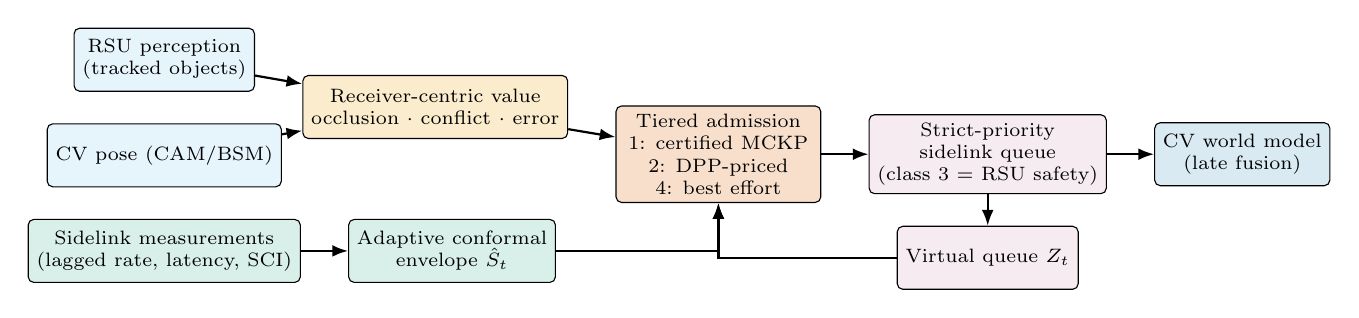
\begin{tikzpicture}[font=\scriptsize,node distance=4mm and 6mm,
  box/.style={draw,rounded corners=2pt,align=center,minimum height=8mm,inner sep=3pt,fill=#1},
  box/.default=white, arr/.style={-{Latex[length=2mm]},thick}]
\node[box=c5!15] (lidar) {RSU perception\\(tracked objects)};
\node[box=c5!15,below=of lidar] (cam) {CV pose (CAM/BSM)};
\node[box=c6!20,right=of lidar,yshift=-6mm] (value) {Receiver-centric value\\occlusion $\cdot$ conflict $\cdot$ error};
\node[box=c3!15,below=of cam] (sci) {Sidelink measurements\\(lagged rate, latency, SCI)};
\node[box=c3!15,right=of sci] (aci) {Adaptive conformal\\envelope $\hat S_t$};
\node[box=c2!20,right=of value,yshift=-6mm,minimum width=26mm] (sched) {Tiered admission\\1: certified MCKP\\2: DPP-priced\\4: best effort};
\node[box=c4!15,right=of sched] (queue) {Strict-priority\\sidelink queue\\(class 3 = RSU safety)};
\node[box=c1!15,right=of queue] (cv) {CV world model\\(late fusion)};
\node[box=c4!15,below=of queue] (z) {Virtual queue $Z_t$};
\draw[arr] (lidar) -- (value); \draw[arr] (cam) -- (value);
\draw[arr] (sci) -- (aci); \draw[arr] (value) -- (sched); \draw[arr] (aci) -| (sched);
\draw[arr] (sched) -- (queue); \draw[arr] (queue) -- (cv); \draw[arr] (queue) -- (z); \draw[arr] (z) -| (sched);
\end{tikzpicture}
\caption{\cs{} at the RSU. Decisions use only RSU tracks, the CV's broadcast pose and lagged sidelink measurements; ground truth is used only offline for evaluation.}
\label{fig:arch}
\end{figure*}

\subsection{Entities and Timing}
An RSU with a roadside LiDAR serves a CV through the sidelink (Fig.~\ref{fig:arch}). Time is divided into decision epochs $t=1,2,\dots$ of length $\Delta=100$~ms aligned with the sensor frames. At epoch $t$ the RSU holds tracked objects $\mathcal I_t$ with world-frame state $s_{i,t}=(x,y,v_x,v_y,l,w,h,\psi,\text{class})$ captured at $c_{i,t}$, and the latest CV pose $p_t$ and velocity $u_t$ received in a cooperative awareness message. After a processing delay $\delta$, the RSU enqueues CPM segments. An update is useful if it arrives within $D$ of capture, i.e., within the relative deadline $\tau=D-\delta$ of the decision.

\subsection{Message Representations}
Each object can be sent in a mode $m\in\mathcal M$ (Table~\ref{tab:modes}). Sizes follow the CPM structure~\cite{etsi103324} with the per-message and per-object sizes used in the CPM literature~\cite{thandavarayan2020generation}. The \emph{kinematic} mode omits the box, so the receiver reconstructs it from a class prior and the heading of motion; the \emph{repetition} mode adds a blind retransmission. Modes therefore change what the receiver knows, and the evaluation recomputes IoU from the transmitted content. A segment carries at most $K$ objects and one header of $H$ bytes.

\begin{table}[t]
\caption{CPM representation modes}\label{tab:modes}\centering\scriptsize
\begin{tabular}{lccc}
\toprule
Mode & Bytes/object & Receiver reconstructs & Copies \\
\midrule
kinematic & 35 & position, velocity; class-prior box & 1\\
box & 60 & position, velocity, box, heading & 1\\
box + repetition & $2\times60$ & as box & 2\\
\midrule
\multicolumn{4}{l}{Header $H=121$~B per segment, at most $K=10$ objects per segment}\\
\bottomrule
\end{tabular}
\end{table}

\subsection{Sidelink Service Model}\label{sec:service}
In window $t$ the sidelink serves the RSU at a gross rate $r_t$ (bytes/ms); each packet experiences an access latency $\ell\le L_t$ drawn from the measured latency distribution of the window and is erased independently with probability $p_t$. Packets are served by strict priority in four classes: (1)~certified critical updates, (2)~priced critical updates, (3)~the RSU's background safety traffic of $A_t$ bytes, and (4)~best-effort updates. Bytes not served by the end of the window are superseded by the next CPM. The bytes deliverable before the deadline at the head of the queue are
\begin{equation}
S_t(\tau)=r_t\,(\tau-L_t)^+ . \label{eq:S}
\end{equation}
\begin{lemma}[Priority delivery]\label{lem:priority}
If the class-1 segments of epoch $t$ total $B^{(1)}_t\le S_t(\tau)$ bytes (headers included) and $\tau\le\Delta$, every class-1 segment is served and arrives within $\tau$ of the decision.
\end{lemma}
\begin{IEEEproof}
Class~1 is served first from the start of the window at rate $r_t$, so its last byte is served at $B^{(1)}_t/r_t\le\tau-L_t\le\Delta$, i.e., inside the window; adding an access latency $\ell\le L_t$ gives arrival at most $\tau$. Packets of earlier epochs do not precede it because they are superseded at the window end.
\end{IEEEproof}

\subsection{Receiver Model and Awareness}
The CV fuses its own detections with received objects (late fusion). For each track it keeps the latest received state, extrapolates it at constant velocity and discards it after $T_{\exp}=1$~s. A ground-truth object is \emph{aware} at time $t'$ if an unexpired received state lies within $d_{\mathrm{m}}=2$~m of it. Objects that the vehicle cannot see itself are \emph{hidden}; hidden objects whose future path comes within 5~m of the CV's future path within 5~s are \emph{critical}. These labels come from ground truth and are used only for evaluation.

\subsection{Problem Formulation}
Let $x_{i,m,t}\in\{0,1\}$ select object $i$ in mode $m$, with value $v_{i,m,t}$ (Section~\ref{sec:value}) and bytes $b_m$. Let $\mathcal C_t\subseteq\mathcal I_t$ be the objects the RSU estimates to be critical, $S^{\mathrm{bg}}_t$ the background bytes served, and $M_t\in\{0,1\}$ indicate that a certified update of epoch $t$ misses its deadline for lack of service. The RSU seeks
\begin{align}
\max_{x}\ & \liminf_{T\to\infty}\frac1T\sum_{t=1}^{T}\sum_{i,m}v_{i,m,t}\,x_{i,m,t} \label{eq:obj}\\
\text{s.t. }& \textstyle\sum_m x_{i,m,t}\le 1, \label{eq:one}\\
& \limsup_{T\to\infty}\tfrac1T\textstyle\sum_{t}M_t\le\alpha, \label{eq:cc}\\
& \liminf_{T\to\infty}\tfrac1T\textstyle\sum_t \big(S^{\mathrm{bg}}_t-\rho A_t\big)\ge 0, \label{eq:bg}
\end{align}
where every decision may use only information available at epoch $t$, and $S_t(\tau)$ is revealed only after the window. Constraint~\eqref{eq:cc} is a chance constraint stated over time, which is the natural reliability notion for a non-stationary channel; \eqref{eq:bg} is the background delivery contract with ratio $\rho$.

% =============================================================================
\section{CertiSched}\label{sec:method}
\subsection{Receiver-Centric Value of an Update}\label{sec:value}
\paragraph*{Ego relevance} The RSU casts five sight lines from $p_t$ to the centre and shrunken corners of each object and counts those blocked by a tall ($\ge1.2$~m) object nearer to the CV; the blocked fraction is the occlusion estimate $o_{i,t}\in[0,1]$, set to 1 beyond the CV sensor range $R$. With both trajectories extrapolated at constant velocity, the closest approach over horizon $H_c$ has distance $d^{\min}_{i,t}$, and $\kappa_{i,t}=e^{-d^{\min}_{i,t}/\sigma_d}$ measures conflict. The relevance weight is
\begin{equation}
w_{i,t}=w_0+(1-w_0)\,o_{i,t}\big(k+(1-k)\kappa_{i,t}\big),
\end{equation}
so a visible object keeps a small weight $w_0$, a hidden object at least $w_0+(1-w_0)k$, and a hidden conflicting object close to 1. Object $i$ is estimated critical ($i\in\mathcal C_t$) if $o_{i,t}\ge o^\star$ and $d^{\min}_{i,t}\le d^\star$.

\paragraph*{Receiver error} Let $\hat s_i$ be the last state the RSU transmitted and $\pi_i$ the probability that it was received (broadcast has no acknowledgement). At the deadline $t+\tau$ the receiver's extrapolation differs from the RSU's prediction by $e^{\mathrm{k}}_{i,t}$; unmodelled acceleration $a_{\max}$ adds $\frac12 a_{\max}\theta^2$ over the belief age $\theta$. We use
\begin{equation}
e_{i,t}=\sqrt{(e^{\mathrm{k}}_{i,t})^2+(\tfrac12a_{\max}\theta^2)^2},\qquad e_{i,t}=\infty\ \text{if}\ \theta\ge T_{\exp},
\end{equation}
and the expected awareness loss $\bar h_{i,t}=\pi_i\big(1-e^{-e_{i,t}/\epsilon}\big)+(1-\pi_i)$.

\paragraph*{Representation fidelity} For the box modes $q_{i,m}=1$; for the kinematic mode $q_{i,m}$ is the bird's-eye-view IoU between the RSU box and its class-prior reconstruction, computed per object.

The value of sending $i$ in mode $m$ under the lagged loss estimate $\hat p_t$ is
\begin{equation}
v_{i,m,t}=w_{i,t}\,\bar h_{i,t}\,\big(1-\hat p_t^{\,c_m}\big)\big(\eta+(1-\eta)q_{i,m}\big). \label{eq:value}
\end{equation}
All terms use RSU-side information only.

\subsection{Adaptive Conformal Service Envelope}\label{sec:envelope}
The scheduler needs a lower bound $\hat S_t$ on $S_t(\tau)$ before window $t$. A quantile gradient-boosting model $f$ maps lagged features $\phi_t$ (rate, latency, loss, channel busy ratio and SCI statistics of windows $t-1,t-2,t-3$ and 10-window summaries) to $S_t(\tau)$; it is trained on other scenarios only (leave-one-scenario-out). With nonconformity $e_u=f(\phi_u)-S_u(\tau)$ and the empirical $(1-\alpha_t)$-quantile $Q_{1-\alpha_t}$ of past scores,
\begin{equation}
\hat S_t=\begin{cases}0,&\alpha_t\le0\\ \big(f(\phi_t)-Q_{1-\alpha_t}(\{e_u\}_{u<t})\big)^+,&0<\alpha_t<1\\ +\infty,&\alpha_t\ge1\end{cases} \label{eq:aci}
\end{equation}
and after observing the window, $\alpha_{t+1}=\alpha_t+\gamma\big(\alpha-\mathrm{err}_t\big)$ with $\mathrm{err}_t=\mathbb 1\{S_t(\tau)<\hat S_t\}$~\cite{gibbs2021aci}. The level rises after covered windows and falls after violations, which re-calibrates the envelope when the channel drifts.

\subsection{Tiered Admission}
Algorithm~\ref{alg:cs} runs each epoch. Class~1 solves the multiple-choice knapsack (MCKP)
\begin{equation}
\max \sum_{i\in\mathcal C_t,m}v_{i,m,t}x_{i,m,t}\ \ \text{s.t.}\ \ \sum_{i,m}b_mx_{i,m,t}+n_tH\le\hat S_t, \label{eq:mckp}
\end{equation}
where $n_t\in\{1,2\}$ headers account for a repetition segment. Critical objects that do not fit are offered to class~2, whose MCKP maximizes $V\sum v\,x-Z_t\sum b\,x$ under the point forecast; the virtual queue
\begin{equation}
Z_{t+1}=\big[Z_t+\rho A_t-S^{\mathrm{bg}}_t\big]^+ \label{eq:z}
\end{equation}
grows when the background is under-served. All remaining objects are planned in class~4 against the point forecast and then appended in value-per-byte order; strict priority lets them use only service left after classes 1--3.

\begin{algorithm}[t]
\caption{\cs{} decision at epoch $t$}\label{alg:cs}
\begin{algorithmic}[1]
\Require tracks $\mathcal I_t$, CV pose, lagged measurements, $Z_t$, $\alpha_t$
\State compute $o_{i,t},\kappa_{i,t},e_{i,t},q_{i,m}$ and $v_{i,m,t}$ by \eqref{eq:value}; split $\mathcal C_t$
\State $\hat S_t\gets$ envelope \eqref{eq:aci}; $\bar S_t\gets$ point forecast
\State class 1: solve \eqref{eq:mckp} on $\mathcal C_t$ (exact DP) $\to\mathcal X^{(1)}$
\State class 2: on $\mathcal C_t\setminus\mathcal X^{(1)}$ maximize $V v-Z_tb$ within $\bar S_t$ $\to\mathcal X^{(2)}$
\State class 4: plan remaining objects within $\bar S_t-A_t$; append the rest by $v/b$
\State enqueue CPM segments; observe $S_t(\tau)$ and $S^{\mathrm{bg}}_t$
\State update $\alpha_{t+1}$ and $Z_{t+1}$ by \eqref{eq:z}
\end{algorithmic}
\end{algorithm}

\subsection{Guarantees}
\begin{theorem}[Certified deadline tier]\label{thm:cert}
For any sequence of service values $\{S_t(\tau)\}$, any base predictor $f$, $\alpha,\alpha_1\in(0,1)$ and $\gamma>0$,
\[
\frac1T\sum_{t=1}^{T}M_t\le\alpha+\frac{\max(\alpha_1,1-\alpha_1)+\gamma}{\gamma T}.
\]
\end{theorem}
\begin{IEEEproof}
Class-1 admission enforces $B^{(1)}_t\le\hat S_t$. If $S_t(\tau)\ge\hat S_t$, Lemma~\ref{lem:priority} delivers every class-1 segment in time; hence $M_t\le\mathrm{err}_t$. Under \eqref{eq:aci}, $\alpha_t\le0$ gives $\hat S_t=0\le S_t(\tau)$ and $\mathrm{err}_t=0$, while $\alpha_t\ge1$ gives $\mathrm{err}_t=1$; therefore $\alpha_t\in[-\gamma,1+\gamma]$ for all $t$ by induction. Summing the update, $\alpha_{T+1}=\alpha_1+\gamma\sum_{t\le T}(\alpha-\mathrm{err}_t)$, so $\frac1T\sum_t M_t\le\frac1T\sum_t\mathrm{err}_t=\alpha+\frac{\alpha_1-\alpha_{T+1}}{\gamma T}\le\alpha+\frac{\alpha_1+\gamma}{\gamma T}$, which is at most the stated bound.
\end{IEEEproof}
\begin{remark}
The bound holds per sample path, without exchangeability or stationarity, which suits a sidelink whose load and geometry drift. Erasures are not service misses; with independent erasures a certified update in mode $m$ is additionally lost with probability $p_t^{c_m}$, which the repetition mode reduces.
\end{remark}

\begin{assumption}\label{ass:slater}
$(r_t,L_t,A_t)$ are i.i.d. over epochs with bounded bytes, and with class-2 traffic switched off the background contract holds with slack $\epsilon>0$: $\mathbb E[S^{\mathrm{bg}}_t-\rho A_t]\ge\epsilon$.
\end{assumption}
\begin{theorem}[Background contract]\label{thm:dpp}
For every sample path, $\frac1T\sum_{t\le T}(\rho A_t-S^{\mathrm{bg}}_t)\le Z_{T+1}/T$. Under Assumption~\ref{ass:slater}, class-2 admission by $\max V\sum v x-Z_t\sum b x$ keeps $\mathbb E[Z_t]=O(V/\epsilon)$, so \eqref{eq:bg} holds, and the class-2 value is within $B/V$ of the best stationary class-2 policy, where $B$ bounds the second moments of the per-epoch bytes.
\end{theorem}
\begin{IEEEproof}
From \eqref{eq:z}, $Z_{t+1}\ge Z_t+\rho A_t-S^{\mathrm{bg}}_t$; summing gives the first claim since $Z_1=0$. Because background is served after classes 1--2 within the window, $S^{\mathrm{bg}}_t\ge S^{\mathrm{bg},0}_t-B^{(2)}_t$, where $S^{\mathrm{bg},0}_t$ is the background service without class~2. The one-step drift $\frac12(Z_{t+1}^2-Z_t^2)$ is therefore at most $B+Z_t(\rho A_t-S^{\mathrm{bg},0}_t)+Z_tB^{(2)}_t$, and subtracting $V\times$value gives the drift-plus-penalty expression whose per-epoch minimizer is the class-2 rule. The remaining steps are those of~\cite[Thm.~4.8]{neely2010book} with the slack of Assumption~\ref{ass:slater}.
\end{IEEEproof}

\begin{proposition}[Solvers]\label{prop:solver}
Rounding byte costs up to a grid $g$, the dynamic program solves each MCKP exactly in $O(|\mathcal I_t||\mathcal M|\lceil \hat S_t/g\rceil)$ time without overstating feasibility. The LP-dominance greedy with the best-single-item safeguard attains at least half of the optimum in $O(|\mathcal I_t||\mathcal M|\log(|\mathcal I_t||\mathcal M|))$~\cite{sinha1979mckp,kellerer2004knapsack}.
\end{proposition}

% =============================================================================
\section{Evaluation Methodology}\label{sec:setup}
\subsection{Data}
\paragraph*{Perception} V2X-Seq-SPD~\cite{v2xseq} provides synchronized roadside and vehicle LiDAR sequences at real intersections with infrastructure-side, vehicle-side and cooperative 3-D labels, track identities and calibration. We use all \resDataSequences{} sequences (\resDataInfrastructureFrames{} infrastructure frames, \resDataVehicleFrames{} vehicle frames). The RSU's perception is the infrastructure-side track annotation, which isolates the scheduling question from detector quality; velocities are causal finite differences. The CV pose comes from its localization. Cooperative labels whose source is the infrastructure only are hidden; among them, \resDataGtCritical{} object-frames are critical by their future paths (\resDataGtHidden{} hidden object-frames in total).
\paragraph*{Sidelink service} SEE-V2X~\cite{seev2x} provides receiver traces and SCI from commercial LTE-V2X radios in perception-only and BSM-plus-perception applications, outdoors at an intersection and indoors over extended durations. Each receiver file is a link; per 100-ms window we extract delivered bytes, loss, channel busy ratio, latency quantiles and SCI statistics (\resDataLinks{} links in \resDataScenarios{} scenarios, \resDataWindows{} windows). The gross service rate is the delivered bytes divided by the window's delivery ratio. Outdoor intersection links form the primary evaluation; indoor links are reported as a secondary condition.
\paragraph*{Pairing} The datasets were not captured together. For each sequence we draw 8~outdoor and 4~indoor link segments with seeded hashes, starting after the envelope's calibration prefix; every policy in a block sees the same objects, CV poses, service, latency draws and erasure draws.

\subsection{Replay}
The replay implements Section~\ref{sec:service}: CPM segments enter the priority queue, are served as a fluid at the window's rate, arrive after a latency drawn from the window's measured quantiles, and are erased with the measured loss. Unserved bytes cost no service and are dropped at the window end. The service of a window is exogenous: the counterfactual RSU may use at most the service that the measured flow obtained, which is conservative where the measured application did not saturate the channel; a CPM-size multiplier sweeps scarcity.

\subsection{Policies}
All baselines run in class~4, after the RSU's background traffic, so that they meet the same contract; their budget is the same point forecast that \cs{} uses for its best-effort tier. \emph{ETSI CPM rules} include objects by the TS~103~324 triggers and order them by time since last inclusion~\cite{etsi103324}. \emph{VoI redundancy mitigation} ranks by confidence $\times$ distance relevance $\times$ novelty~\cite{lyu2025voi}. \emph{Max-weight AoI} ranks by $(1-\hat p_t)\theta(\theta+\Delta)$~\cite{kadota2018}. \emph{Confidence density} ranks by confidence per byte, the object-level analogue of Where2comm~\cite{where2comm}. \emph{Send all} transmits every object in box mode. As sensitivity, AoI and VoI also run in class~2, ahead of the background. \emph{Oracle service} is \cs{} with $\hat S_t=S_t(\tau)$ (not causal). Ablations remove one component at a time (Table~\ref{tab:ablation}).

\subsection{Metrics and Statistics}
Primary: critical awareness and hidden awareness, i.e., the fraction of (object, vehicle frame) pairs that are aware. Secondary: AoI of aware critical objects, AP of the fused object list at BEV IoU 0.5 and 3-D IoU 0.7 (car classes), background delivery ratio $\sum S^{\mathrm{bg}}/\sum A$, sidelink load, the certified miss frequency of Theorem~\ref{thm:cert} (epochs with a class-1 service miss over all epochs), and decision time. The road sequence is the statistical unit: run outcomes are averaged per sequence and 95\% intervals use 5,000 cluster-bootstrap resamples~\cite{cameron2008}. The confirmatory family, fixed before the data run, compares \cs{} with each contract-compliant baseline on the two primary metrics (Wilcoxon signed-rank on sequence means~\cite{wilcoxon1945}, Holm correction~\cite{holm1979}). Table~\ref{tab:params} lists all parameters.

\begin{table}[t]
\caption{Parameters (all varied in sensitivity studies where noted)}\label{tab:params}\centering\scriptsize
\begin{tabular}{ll}
\toprule
Epoch $\Delta$, processing $\delta$, deadline $D$ ($\tau$) & 100, 20, 100 (80) ms\\
Certified target $\alpha$ (sweep) & 0.05 (0.01--0.20)\\
ACI step $\gamma$, score window, calibration prefix & 0.005, 2000, 20\%\\
Background contract $\rho$, DPP $V$ (sweep) & 0.95, $10^6$ ($10^4$--$10^7$)\\
Background traffic $A_t$ & 2 streams $\times$ 300 B per 100 ms\\
CV sensor range $R$, conflict horizon $H_c$, $\sigma_d$ & 60 m, 5 s, 5 m\\
Critical estimate $o^\star$, $d^\star$ & 0.5, 8 m\\
$w_0$, $k$, $\epsilon$, $\eta$, $a_{\max}$, $T_{\exp}$ & 0.05, 0.3, 1 m, 0.5, 1.5 m/s$^2$, 1 s\\
CPM sizes, segment size $K$ (load sweep) & Table~\ref{tab:modes}, 10 ($\times$1, 2, 4)\\
\bottomrule
\end{tabular}
\end{table}

% =============================================================================
\section{Results}\label{sec:results}
\subsection{Calibration of the Service Envelope}
Fig.~\ref{fig:calib} evaluates the envelopes on every held-out window, without any controller. The point forecast is exceeded in \resEnvPointMiss{} of windows and the last-value rule in \resEnvLastMiss{}, so a budget set from a forecast fails about half of the time. For $\alpha=0.05$ the adaptive envelope misses in \resEnvAciAZeroFiveMiss{} of windows, compared with \resEnvSplitAZeroFiveMiss{} for split conformal and \resEnvRollingAZeroFiveMiss{} for fixed-level rolling conformal, and it retains a fraction \resEnvAciAZeroFiveEff{} of the mean deliverable bytes.

\begin{figure}[t]
\centering
\csvplot{envelope_calibration.csv}{%
\begin{tikzpicture}
\begin{groupplot}[group style={group size=2 by 1,horizontal sep=12mm},width=0.53\linewidth,height=40mm]
\nextgroupplot[xmode=log,ymode=log,xlabel={target $\alpha$},ylabel={window miss frequency},title={(a) calibration},legend pos=north west]
\addplot[gray,dashed,domain=0.008:0.25] {x}; \addlegendentry{ideal}
\addplot[c1,mark=*,thick] table[col sep=comma,x=alpha,y=miss]{\resdir/fig_calib_aci.csv}; \addlegendentry{ACI}
\addplot[c2,mark=square*,thick] table[col sep=comma,x=alpha,y=miss]{\resdir/fig_calib_split.csv}; \addlegendentry{split}
\addplot[c3,mark=triangle*,thick] table[col sep=comma,x=alpha,y=miss]{\resdir/fig_calib_rolling.csv}; \addlegendentry{rolling}
\nextgroupplot[xmode=log,xlabel={target $\alpha$},ylabel={bound / mean service},title={(b) efficiency}]
\addplot[c1,mark=*,thick] table[col sep=comma,x=alpha,y=efficiency]{\resdir/fig_calib_aci.csv};
\addplot[c2,mark=square*,thick] table[col sep=comma,x=alpha,y=efficiency]{\resdir/fig_calib_split.csv};
\addplot[c3,mark=triangle*,thick] table[col sep=comma,x=alpha,y=efficiency]{\resdir/fig_calib_rolling.csv};
\end{groupplot}
\end{tikzpicture}}
\caption{Controller-free envelope evaluation on all held-out windows of the measured links: (a) empirical miss frequency versus target; (b) mean bound relative to mean deliverable bytes.}
\label{fig:calib}
\end{figure}

\subsection{Main Comparison}
Table~\ref{tab:main} reports the primary (outdoor) condition and Table~\ref{tab:tests} the confirmatory tests. \cs{} reaches a critical awareness of \resCertischedCriticalAwareness{} and a hidden awareness of \resCertischedHiddenAwareness{}, against \resEtsiCpmRulesCriticalAwareness{} and \resEtsiCpmRulesHiddenAwareness{} for ETSI CPM rules, \resVoiRedundancyMitigationCriticalAwareness{} and \resVoiRedundancyMitigationHiddenAwareness{} for VoI redundancy mitigation, and \resMaxWeightAoiCriticalAwareness{} and \resMaxWeightAoiHiddenAwareness{} for max-weight AoI. The mean age of the critical objects the vehicle knows is \resCertischedAoi{}~ms (ETSI: \resEtsiCpmRulesAoi{}~ms). The certified miss frequency is \resCertischedCertWindowMiss{} for a target of 0.05, and the background delivery ratio is \resCertischedBackgroundDelivery{}. The oracle variant, which knows each window's service, reaches \resOracleServiceCriticalAwareness{}, which bounds what better service prediction alone could add.

\begin{table*}[t]
\caption{Primary condition (outdoor intersection links). Sequence-level means with 95\% cluster-bootstrap intervals; AP of the fused list for car classes}\label{tab:main}
\centering\scriptsize
\resizebox{\textwidth}{!}{%
\begin{tabular}{lcccccccc}
\toprule
Policy & Critical awareness & Hidden awareness & Crit. AoI (ms) & AP$_{\mathrm{BEV}}$@0.5 & AP$_{\mathrm{3D}}$@0.7 & Background & Load (kbit/s) & Cert. miss \\
\midrule
\resultinput{table_main_rows.tex}
\bottomrule
\end{tabular}}
\end{table*}

\begin{table}[t]
\caption{Confirmatory tests: \cs{} minus baseline (sequence means, Holm-adjusted)}\label{tab:tests}
\centering\scriptsize
\resizebox{\columnwidth}{!}{%
\begin{tabular}{llcccc}
\toprule
Baseline & Metric & $\Delta$ & 95\% CI & Fav. & $p_{\mathrm{Holm}}$\\
\midrule
\resultinput{table_tests_rows.tex}
\bottomrule
\end{tabular}}
\end{table}

\subsection{Ablations}
Table~\ref{tab:ablation} removes one component at a time. Replacing the conformal envelope by the point forecast raises the certified miss frequency to \resWOConformalPointCertWindowMiss{}; split and fixed-level conformal keep the average level but lose calibration where the link drifts (Fig.~\ref{fig:calib}). Removing ego relevance or tiers lowers critical awareness to \resWOEgoRelevanceCriticalAwareness{} and \resWOTiersCriticalAwareness{}; removing the best-effort tier lowers hidden awareness to \resWOOpportunisticTierHiddenAwareness{}; removing the DPP queue changes the background ratio to \resWODppBackgroundDelivery{}.

\begin{table*}[t]
\caption{Ablations (primary condition)}\label{tab:ablation}
\centering\scriptsize
\resizebox{\textwidth}{!}{%
\begin{tabular}{lcccccccc}
\toprule
Variant & Critical awareness & Hidden awareness & Crit. AoI (ms) & AP$_{\mathrm{BEV}}$@0.5 & AP$_{\mathrm{3D}}$@0.7 & Background & Load (kbit/s) & Cert. miss \\
\midrule
\resultinput{table_ablation_rows.tex}
\bottomrule
\end{tabular}}
\end{table*}

\subsection{Trade-offs and Scarcity}
Fig.~\ref{fig:sweeps} shows the effect of the DPP parameter $V$, the certified target $\alpha$ and channel scarcity. Larger $V$ admits more priced critical traffic at the expense of background delivery, as Theorem~\ref{thm:dpp} predicts. The certified miss frequency stays below each target $\alpha$ (Theorem~\ref{thm:cert}). As CPM sizes grow, every policy loses awareness; the gap between \cs{} and the baselines indicates how much of the scarce service each policy spends on objects the vehicle needs.

\begin{figure*}[t]
\centering
\csvplot{fig_alpha_sweep.csv}{%
\begin{tikzpicture}
\begin{groupplot}[group style={group size=3 by 1,horizontal sep=14mm},width=0.32\textwidth,height=42mm]
\nextgroupplot[xmode=log,xlabel={$V$},ylabel={ratio},title={(a) DPP trade-off},legend pos=south west]
\addplot[c1,mark=*,thick] table[col sep=comma,x=p_v_dpp,y=critical_awareness]{\resdir/fig_v_sweep.csv}; \addlegendentry{critical awareness}
\addplot[c2,mark=square*,thick] table[col sep=comma,x=p_v_dpp,y=background_delivery]{\resdir/fig_v_sweep.csv}; \addlegendentry{background}
\nextgroupplot[xmode=log,ymode=log,xlabel={target $\alpha$},ylabel={certified miss frequency},title={(b) certified tier}]
\addplot[gray,dashed,domain=0.008:0.25] {x};
\addplot[c1,mark=*,thick] table[col sep=comma,x=p_alpha_crit,y=cert_window_miss]{\resdir/fig_alpha_sweep.csv};
\nextgroupplot[xlabel={CPM size multiplier},ylabel={critical awareness},title={(c) scarcity},legend pos=north east,xtick={1,2,4}]
\addplot[c1,mark=*,thick] table[col sep=comma,x=load_factor,y=certisched]{\resdir/fig_load_critical_awareness.csv}; \addlegendentry{\cs}
\addplot[c2,mark=square*,thick] table[col sep=comma,x=load_factor,y=etsi]{\resdir/fig_load_critical_awareness.csv}; \addlegendentry{ETSI}
\addplot[c3,mark=triangle*,thick] table[col sep=comma,x=load_factor,y=voi]{\resdir/fig_load_critical_awareness.csv}; \addlegendentry{VoI}
\addplot[c4,mark=diamond*,thick] table[col sep=comma,x=load_factor,y=aoi]{\resdir/fig_load_critical_awareness.csv}; \addlegendentry{AoI}
\addplot[gray,dashed,mark=o] table[col sep=comma,x=load_factor,y=oracle]{\resdir/fig_load_critical_awareness.csv}; \addlegendentry{oracle}
\end{groupplot}
\end{tikzpicture}}
\caption{(a) DPP parameter $V$; (b) certified miss frequency versus target; (c) critical awareness versus CPM size multiplier (primary condition).}
\label{fig:sweeps}
\end{figure*}

\subsection{Secondary Condition and Computation}
On indoor extended-duration links (Table~\ref{tab:secondary}) service is richer and steadier, so differences between policies shrink. A decision takes \resCertischedDecisionMs{}~ms on average in single-threaded Python on a laptop CPU with the exact dynamic program, far below the 100-ms epoch; the greedy variant (Proposition~\ref{prop:solver}) is faster with a guaranteed half-optimal objective.

\begin{table*}[t]
\caption{Secondary condition (indoor extended-duration links)}\label{tab:secondary}
\centering\scriptsize
\resizebox{\textwidth}{!}{%
\begin{tabular}{lcccccccc}
\toprule
Policy & Critical awareness & Hidden awareness & Crit. AoI (ms) & AP$_{\mathrm{BEV}}$@0.5 & AP$_{\mathrm{3D}}$@0.7 & Background & Load (kbit/s) & Cert. miss \\
\midrule
\resultinput{table_secondary_rows.tex}
\bottomrule
\end{tabular}}
\end{table*}

% =============================================================================
\section{Discussion and Limitations}
\paragraph*{What the guarantee covers} Theorem~\ref{thm:cert} bounds service-induced misses of the certified tier over time for any service sequence. It does not bound erasures, which the repetition mode reduces under an independence assumption, and it does not promise that every critical object is certified: when the envelope is small, the remaining critical objects go to class~2 or class~4 without a guarantee, and the tables report their outcomes.
\paragraph*{Service-capped replay} The counterfactual RSU never uses more service than the measured application obtained in that window, which is conservative when the application did not saturate the channel. The datasets were not captured together, so road geometry does not influence the channel; the sweeps over scarcity and the two measurement conditions bound this effect but do not remove it. Over-the-air validation with commercial radios is the next step.
\paragraph*{Perception} Using infrastructure annotations as RSU perception isolates scheduling from detection errors; a learned detector would add false and missed objects that affect all policies alike, and the value function accepts detector confidence through $\pi_i$ and the VoI baseline's accuracy term.
\paragraph*{Single receiver} V2X-Seq-SPD has one CV per sequence. With several receivers, the value becomes a sum over receivers of \eqref{eq:value}, and the admission problem keeps its form because a broadcast object is sent once.

\section{Conclusion}
\cs{} turns the RSU's CPM decision into a receiver-centric, risk-tiered scheduling problem and gives its most critical tier a distribution-free deadline guarantee calibrated online from sidelink measurements, while a virtual queue protects the RSU's own safety traffic. On real perception sequences and real C-V2X service it delivers higher awareness of hidden, conflicting objects than standardized and age-based baselines under the same service contract, at negligible computational cost. Future work will validate the scheduler over the air, extend it to several receivers and to NR-V2X Mode~2.

\section*{Data and Code Availability}
V2X-Seq-SPD and SEE-V2X are available from their providers~\cite{v2xseq,seev2x}. The artifact contains the full pipeline, configuration, tests and all aggregate results; raw data are not redistributed.

\bibliographystyle{IEEEtran}
\bibliography{refs}

\end{document}
